\documentclass[margin=1pt]{standalone}
\usepackage{color,xcolor}
\usepackage{makecell}
\usepackage{tikz-qtree, tikz}
\usepackage[utf8]{inputenc}


\begin{document}
\begin{tikzpicture}
    \node[anchor=south west,inner sep=0] (graph) at (0,0) {
        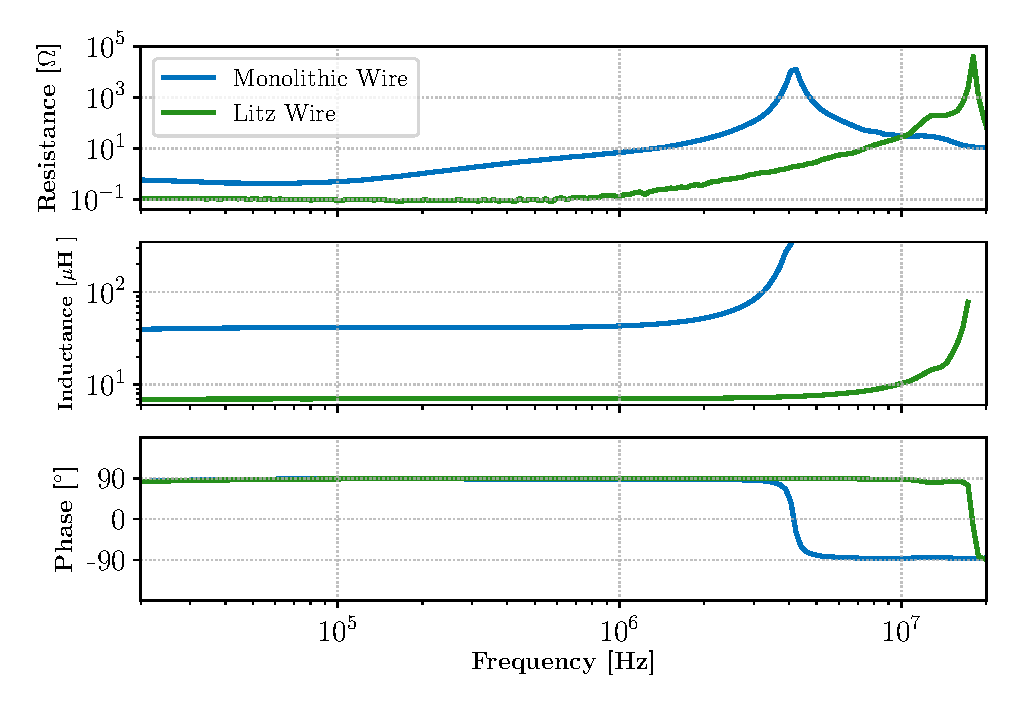
\includegraphics{impedance-analysis-graph.pdf}
    };
    \begin{scope}[x={(graph.south east)},y={(graph.north west)}]
        \node[anchor=center,inner sep=0,scale=1.75] (image-wires) at (0.55,1.15) {
            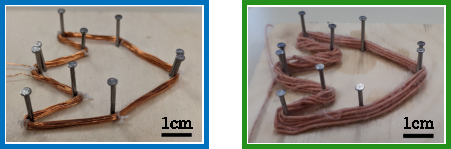
\includegraphics{induction-heating-wires.pdf}
        };
        \draw[ultra thick] (0.775,0.154) node[yshift=-12] {\large $f_c^\mathrm{mono}$} -- (0.775,0.935);
        \draw[ultra thick] (0.95,0.154) node[yshift=-12] {\large $f_c^\mathrm{litz}$} -- (0.95,0.935);
        % \node [anchor=center, rotate=90] (ylabel) at (1,0.5) {\normalsize Temperature [$^\circ$C]};
      % \draw[help lines,xstep=.05,ystep=.05] (0,0) grid (1,1);
      %   \foreach \x in {0,1,...,9} { \node [anchor=north] at (\x/10,0) {0.\x}; }
      %   \foreach \y in {0,1,...,9} { \node [anchor=east] at (0,\y/10) {0.\y}; }
    \end{scope}
\end{tikzpicture}
\end{document}
